\paragraph{\trBifibration{}。}\label{sub:bifibrations}
现在我们来看如下类型的图：
\begin{equation}\label{eq:bifibration-diagram}
\begin{tikzcd}[column sep=large]
\scr{E} \ar[r,"\varpi"] \ar[rr,bend left=16,"{\Psi=\psi\circ\varpi}"]
 & \scr{S} \ar[r,"\psi"] & \scr{W}.
\end{tikzcd}
\end{equation}
这里 $\Psi$ 是一个\trLefschetzFibration，其\trTotalSpace{}的维数为
$2n+4\ge 6$。中间空间 $\scr{S}$ 是一个\trCorneredBoundary{}的%
\trExactSymplectic{}四维\trManifold，而 $\varpi$ 与 $\psi$ 都是%
\trFibrationWithSingularities{}。对 $\psi$，我
们假定它没有\trCriticalPoint，并且它的\trFiber{}是带边界的%
\trConnected\trSurface{}（特别地，$\scr{S}$ 只有\trCodimension{}$\le 2$ 的角）。对
$\varpi$，我们只要求它在 $\partial^h\scr{S}$ 上没有\trCriticalValue，这里的
这一部分边界是相对于 $\psi$ 定义的。取一点 $w\in\scr{W}$，把
$\varpi$ 限制到位于该点之上的那些\trFiber{}上，所得结果记作
\begin{equation}\label{eq:fibre-over-point}
\scr{E}_w\xrightarrow{\ \varpi_w\ }\scr{S}_w,
\end{equation}
只要 $w$ 不是 $\Psi$ 的\trCriticalValue{}之一，它就是一个%
\trFibrationWithSingularities{}（其余一切必需的性质都可由关于 $\varpi$、$\psi$ 与 $\Psi$ 的
假设推出）。因此可以把 $\scr{E}\to\scr{W}$ 想成这样一个\trLefschetzFibration：
其\trSmooth\trFiber{}又逐张地\trFibration{}在\trSurface{}$\scr{S}_w$ 之上。若 \eqref{eq:bifibration-diagram}
还满足下列附加条件，我们就称之为一个\textbf{\trLefschetz\trBifibration}
（(exact) Lefschetz bifibration）：
\begin{itemize}
\item $\varpi$ 的\trCriticalPoint{}是\trGeneric{}的，其含义是：$D\varpi$ 在
$\Hom_\CC(T\scr{E},\varpi^*T\scr{S})$ 中既与\trZeroSection{}\trTransverse，
也与由复秩 $1$ 的\trLinear{}映射组成的\trStratum{}\trTransverse。若 $x$ 是
$\varpi$ 的\trCriticalPoint{}但却是 $\Psi$ 的\trRegular{}点，则 $I_{\scr{E}}$
限制在\trFiber{}$\scr{E}_w$（$w=\Psi(x)$）上在 $x$ 附近局部可积。而且，对每个
$w\in\partial\scr{W}$，\eqref{eq:fibre-over-point} 都是一个\trLefschetzFibration。
\item 取 $w\in\mathrm{Critv}(\Psi)$，并设 $x$ 是 $\scr{E}_w$ 中那个唯一的%
\trCriticalPoint。我们要求 $D^2\Psi_x$ 限制在 $\ker(D\varpi_x)\subset
T\scr{E}_x$ 上是\trNondegenerate{}的。\trAlmostComplex{}结构 $I_{\scr{S}}$ 在
$\varpi(x)$ 的一个邻域内可积。而且，$\varpi_w$ 落在 $\scr{E}_w\setminus\{x\}$
上的全部\trCriticalPoint{}都必须\trNondegenerate，其 $\varpi$-值两两不同，
并且也都不同于 $\varpi(x)$。
\end{itemize}
现在我们来逐步解开这套条件的含义。\trGenericity{}与维数计数表明 $D\varpi$
永不为零，而使它具有 $\CC$-秩 $1$ 的点集 $\mathrm{Crit}(\varpi)$ 是一个%
\trSmooth
的二维\trSubmanifold。事实上，
\begin{lemma}\label{thm:crit-curve-holomorphic}
$\mathrm{Crit}(\varpi)$ 是一条\trSmooth{}的 $I_{\scr{E}}$-\trHolomorphic{}曲线。
\end{lemma}
\begin{proof}
取 $x\in\mathrm{Crit}(\varpi)$ 与 $X\in T\scr{E}_x$，考虑偏二阶导数
\begin{equation}\label{eq:partial-second-derivative}
\bar{D}^2\varpi_{x,X}\colon\ker(D\varpi_x)\longrightarrow
\mathrm{coker}(D\varpi_x).
\end{equation}
$\mathrm{Crit}(\varpi)$ 的\trTangentSpace{}由使它为零的那些 $X$ 组成。在局
部坐标里作一个简单的计算可知
$\bar{D}^2\varpi_{x,I_{\scr{E}}X}=I_{\scr{S}}\bar{D}^2\varpi_{x,X}$。
\end{proof}
\begin{lemma}\label{thm:crit-intersection-transverse}
设 $x$ 是 $\mathrm{Crit}(\varpi)\setminus\mathrm{Crit}(\Psi)$ 中的一点，且
$\Psi(x)=w$。那么 $x$ 是 $\varpi_w$ 的一个\trCriticalPoint；并且，
$\mathrm{Crit}(\varpi)\cap\scr{E}_w$ 在 $x$ 处\trTransverse，当且仅当它作为
$\varpi_w$ 的\trCriticalPoint{}是\trNondegenerate{}的。\footnote{译注：原书
此处印作“$\mathrm{Crit}(\varpi)\cap E_w$”（斜体 $E$）；按本节记号及下文证
明疑应为\trFiber{}$\scr{E}_w$（花体）；此处径改。——译者注}
\end{lemma}
\begin{proof}
由于 $x$ 不是 $\Psi$ 的\trCriticalPoint，$D\varpi_x$ 的像与 $\scr{S}_w$ 的%
\trTangentSpace{}\trTransverse。这意味着 $\ker(D\varpi_x)=T(\scr{E}_w)_x$，
并且由\trInclusionMap{}诱导的映射 $T(\scr{S}_w)_x\to\mathrm{coker}(D\varpi_x)$
是一个\trIsomorphism。由此得出 $D(\varpi_w)_x=0$，而且对
$X\in T(\scr{E}_w)_x$，可以把 \eqref{eq:partial-second-derivative} 等同于通
常的二阶导数 $D^2(\varpi_w)_{x,X}$。若交 $\mathrm{Crit}(\varpi)\cap\scr{E}_w$
是\trTransverse{}的，则 \eqref{eq:partial-second-derivative} 对任何非零的
$X\in T(\scr{E}_w)_x$ 都必须非零，这就意味着该\trCriticalPoint{}是%
\trNondegenerate{}的。同一论证给出逆命题。
\end{proof}
\begin{lemma}\label{thm:crit-local-embedding}
在 $\Psi$ 的每个\trCriticalPoint{}$x$ 处，映射
$\varpi|\mathrm{Crit}(\varpi)\colon\mathrm{Crit}(\varpi)\to\scr{S}$ 是一个局
部\trEmbedding，而 $\Psi|\mathrm{Crit}(\varpi)\colon\mathrm{Crit}(\varpi)\to\scr{W}$
有一个 $2$ 阶\trBranchPoint。
\end{lemma}
\begin{proof}
由于 $D\varpi_x$ 的秩为 $1$ 而 $D\Psi_x$ 恒为零，$D\psi_{\varpi(x)}$ 把
$\mathrm{coker}(D\varpi_x)$ \trIsomorphic{}地映到 $T\scr{W}_w$（$w=\Psi(x)$）
上。在这一等同之下，\eqref{eq:partial-second-derivative} 就成为 $\Psi$ 在
$x$ 处通常的二阶导数，这意味着 $\mathrm{Crit}(\varpi)$ 的\trTangentSpace{}
在 $\CC$ 上由一个非零的 $X$ 生成，后者满足：对一切 $Y\in\ker(D\varpi_x)$ 都
有 $D^2\Psi_x(X,Y)=0$。我们已假定 $D^2\Psi_x$ 在 $\ker(D\varpi_x)$ 上%
\trNondegenerate；于是 $D\varpi_x(X)\neq 0$，这就证明了我们的第一个断言。
\trNondegenerate{}性假设还蕴含 $D^2\Psi_x(X,X)\neq 0$，这表明
$\Psi|\mathrm{Crit}(\varpi)$ 在 $x$ 处的二阶导数非零。
\end{proof}
\begin{lemma}\label{thm:bifibration-normal-form}
在 $\Psi$ 的每个\trCriticalPoint{}及其在 $\scr{S}$、$\scr{W}$ 中的值附近，
都存在局部\trHolomorphic{}坐标，使得
\begin{equation*}
\varpi(x_1,\dots,x_{n+2})=(x_1^2+x_2^2+\cdots+x_{n+2}^2,\,x_1),
\qquad \psi(y_1,y_2)=y_1.
\end{equation*}
\end{lemma}
\begin{proof}
这是\trHolomorphic\trMorseLemma{}的\trParametrization{}版本的推论（其证明与
非\trParametrization{}情形相同）。
先在 $\scr{S}$ 与 $\scr{W}$ 上引进\trHolomorphic{}局部坐标，以我们这个\trCriticalPoint{}
的 $\varpi$-值与 $\Psi$-值为中心，使 $\psi$ 在其中具有所要求的形式
$\psi(y_1,y_2)=y_1$（这是做得到的，因为按假设 $I_{\scr{S}}$ 局部可积）。在
这些坐标里局部地把 $\varpi$ 写成 $\varpi=(\varpi_1,\varpi_2)\colon\scr{E}\to
\CC^2$，可以发现 $D\varpi_2$ 在该\trCriticalPoint{}处非零，因此\trLevelSet
$\{\varpi_2=0\}$ \trSmooth，而且 $\varpi_1=\Psi$ 限制在该\trLevelSet{}上时
在 $x$ 处有
一个\trNondegenerate{}\trCriticalPoint。由此，邻近的\trLevelSet{}
$\{\varpi_2=y_2\}$
也都\trSmooth，而 $\varpi_1$ 限制在其中每一张上都有一个单独的\trNondegenerate%
\trCriticalPoint，它\trHolomorphic{}地依赖于 $y_2$。于是可以在每张%
\trLevelSet{}上找到\trHolomorphic{}地依赖于 $y_2$ 的局部坐标
$x_2,\dots,x_{n+2}$，使 $\varpi_1$ 限制在该\trLevelSet{}上具
有通常的二次正规形式。再添上 $x_1=\varpi_2$，就得到\trTotalSpace{}上的一个
坐标集%
\footnote{译注：原书此处印作“a coordinate set on $E$”（斜体 $E$）；按本节
记号疑应为\trTotalSpace{}$\scr{E}$；此处径改。——译者注}，使得
$\varpi(x_1,\dots,x_{n+2})=(f(x_1)+x_2^2+\cdots+x_{n+2}^2,\,x_1)$，其中 $f$
是某个\trHolomorphic{}函数。按假设，$x=0$ 是 $\varpi_1=\Psi$ 的一个\trNondegenerate%
\trCriticalPoint，故对某个 $c\neq 0$ 有 $f(t)=ct^2+O(t^3)$。最后一步，把
$x_1$ 换成 $f^{1/2}(x_1)$，并把 $y_2$ 换成 $f^{1/2}(y_2)$。
\end{proof}
现在我们来讨论这些技术性结果对临界曲线及其像的几何而言意味着什么。
\begin{equation*}
\begin{tikzcd}[column sep=large]
\mathrm{Crit}(\varpi) \ar[r,"\varpi|\mathrm{Crit}(\varpi)"]
 \ar[rr,bend left=15,"\Psi|\mathrm{Crit}(\varpi)"]
 & \mathrm{Critv}(\varpi) \ar[r,"\psi|\mathrm{Critv}(\varpi)"] & \scr{W}.
\end{tikzcd}
\end{equation*}
由于已经假定 $\mathrm{Critv}(\varpi)\cap\partial^h\scr{S}=\varnothing$，
$\mathrm{Crit}(\varpi)$ 的边界就等于它与 $\Psi^{-1}(\partial\scr{W})$
的交；又因 $\phi_{\scr{E}}$ 是\trExact{}的，$\mathrm{Crit}(\varpi)$ 的每个%
\trConnectedComponent{}都必定带有边界。这蕴含：没有任何分支能整个包含在
$\Psi$ 的一条\trFiber{}里，从而 $\Psi|\mathrm{Crit}(\varpi)$ 是一个有限的%
\trBranchedCover。据\cref{thm:crit-intersection-transverse}，对
$w\in\partial\scr{W}$ 要求 $\varpi_w$ 为\trLefschetzFibration{}就意味着：在
$\partial\mathrm{Crit}(\varpi)$ 的某个邻域内，$\varpi|\mathrm{Crit}(\varpi)$
是\trEmbedding，而 $\Psi|\mathrm{Crit}(\varpi)$ 是局部\trIsomorphism。应用一些基本的%
\trPseudoholomorphicCurve{}理论可以看到，$\varpi|\mathrm{Crit}(\varpi)$ 几乎
处处\trInjective，故其像 $\mathrm{Critv}(\varpi)$ 是一条不含\trMultipleCover{}分支
的 $I_{\scr{S}}$-\trHolomorphic{}曲线。此外，在它的边界
$\partial\mathrm{Critv}(\varpi)=\mathrm{Critv}(\varpi)\cap\partial^v\scr{S}$
附近，这条曲线是\trSmooth{}的，而 $\psi|\mathrm{Critv}(\varpi)$ 是局部\trIsomorphism。%
\cref{thm:crit-intersection-transverse}与\cref{thm:crit-local-embedding}相结
合表明：对 $w\in\mathrm{Crit}(\Psi)$，$\mathrm{Critv}(\varpi)$ 在 $\scr{S}_w$
的某个邻域内也是\trSmooth{}的，而且每张这样的 $\scr{S}_w$ 都含有
$\psi|\mathrm{Critv}(\varpi)$ 的单个\trBranchPoint，并且其阶为 $2$。%
\cref{fig:bifibration-summary}总结了这一局面。
\begin{figure}[htbp]
\centering
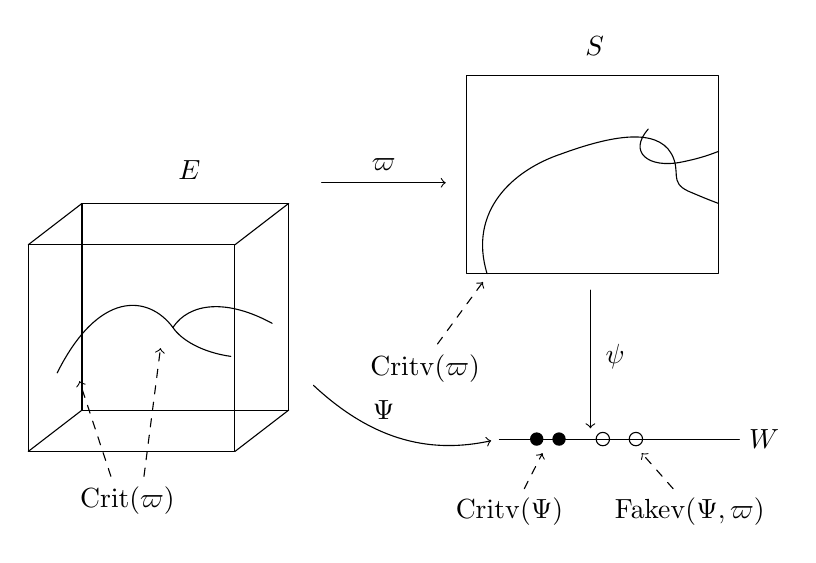
\begin{tikzpicture}[line cap=round,line join=round,scale=1.05]
\draw (0,0) rectangle (2.5,2.5);
\draw (0.65,0.5) rectangle (3.15,3.0);
\draw (0,0) -- (0.65,0.5) (2.5,0) -- (3.15,0.5) (2.5,2.5) -- (3.15,3.0)
      (0,2.5) -- (0.65,3.0);
\node at (1.95,3.4) {$\scr{E}$};
\draw (0.35,0.95) .. controls (0.85,1.95) and (1.45,1.9) .. (1.75,1.5);
\draw (1.75,1.5) .. controls (1.95,1.8) and (2.4,1.85) .. (2.95,1.55);
\draw (1.75,1.5) .. controls (1.85,1.35) and (2.1,1.2) .. (2.45,1.15);
\draw[dashed,->] (1.0,-0.3) -- (0.62,0.85);
\draw[dashed,->] (1.4,-0.3) -- (1.6,1.25);
\node at (1.2,-0.6) {$\mathrm{Crit}(\varpi)$};
\draw[->] (3.55,3.25) -- (5.05,3.25);
\node at (4.3,3.47) {$\varpi$};
\draw (5.3,2.15) rectangle (8.35,4.55);
\node at (6.85,4.9) {$\scr{S}$};
\draw (5.55,2.15) .. controls (5.32,2.9) and (5.85,3.4) .. (6.45,3.6)
                 .. controls (7.05,3.82) and (7.6,3.92) .. (7.78,3.6)
                 .. controls (7.9,3.38) and (7.75,3.26) .. (7.98,3.15)
                 .. controls (8.12,3.09) and (8.24,3.04) .. (8.35,3.0);
\draw (7.5,3.9) .. controls (7.25,3.62) and (7.5,3.42) .. (7.9,3.5)
               .. controls (8.15,3.55) and (8.27,3.6) .. (8.35,3.63);
\draw[dashed,->] (4.95,1.3) -- (5.5,2.05);
\node at (4.8,1.0) {$\mathrm{Critv}(\varpi)$};
\draw[->] (6.8,1.95) -- (6.8,0.28);
\node at (7.1,1.15) {$\psi$};
\draw (5.7,0.15) -- (8.6,0.15);
\node at (8.9,0.15) {$\scr{W}$};
\fill (6.15,0.15) circle (2.3pt);
\fill (6.42,0.15) circle (2.3pt);
\draw (6.95,0.15) circle (2.3pt);
\draw (7.35,0.15) circle (2.3pt);
\draw[dashed,->] (6.0,-0.45) -- (6.22,-0.02);
\node at (5.82,-0.73) {$\mathrm{Critv}(\Psi)$};
\draw[dashed,->] (7.8,-0.45) -- (7.42,-0.02);
\node at (8.0,-0.73) {$\mathrm{Fakev}(\Psi,\varpi)$};
\draw[->] (3.45,0.8) .. controls (4.2,0.1) and (4.9,-0.02) .. (5.6,0.13);
\node at (4.3,0.5) {$\Psi$};
\end{tikzpicture}
\caption{}\label{fig:bifibration-summary}
\end{figure}
我们定义\textbf{\trFakeCriticalValue}（fake critical value）集
$\mathrm{Fakev}(\Psi,\varpi)$ 为由那些 $w\in\scr{W}\setminus\mathrm{Critv}(\Psi)$
组成的集合：它们使得 $\mathrm{Critv}(\varpi)$ 或者有\trSingularPoint{}落在
$\scr{S}_w$ 上，或者在 $\scr{S}_w$ 附近\trSmooth、却以非\trTransverse{}的方
式与它相交。换个与之\trEquivalence{}的说法：这些就是使 $\scr{E}_w$
\trSmooth、而 \eqref{eq:fibre-over-point}
却不成其为\trLefschetzFibration{}的那些 $w$。据前文的讨论，
$\mathrm{Fakev}(\Psi,\varpi)$ 是 $\mathrm{int}(\scr{W})$ 的有限子集；特别
地，$\scr{W}\setminus(\mathrm{Critv}(\Psi)\cup\mathrm{Fakev}(\Psi,\varpi))$
依然是\trConnected{}的。
